\documentclass[11pt]{article}

\usepackage[hyphens]{url}

\usepackage[document]{ragged2e}

\usepackage{hyperref}
\hypersetup
{
    breaklinks = true,
    allcolors = black,
    linktoc = all
}

\usepackage{mathtools}
\usepackage{amssymb}
\usepackage{stmaryrd}
\usepackage{graphicx}

\usepackage{multicol}
\setlength{\columnseprule}{0.4pt}

\usepackage{listings}
\lstloadlanguages{Haskell}
\lstset
{
    escapeinside={(*@}{@*)},
    basicstyle=\small\ttfamily,
    flexiblecolumns=false,
    basewidth={0.5em,0.45em},
    literate={+}{{$+$}}1 {/}{{$/$}}1 {*}{{$*$}}1 {=}{{$=$}}1
            {>}{{$>$}}1 {<}{{$<$}}1 {\\}{{$\lambda$}}1
            {\\\\}{{\char`\\\char`\\}}1
            {->}{{$\rightarrow$}}2 {>=}{{$\geq$}}2 {<-}{{$\leftarrow$}}2
            {<=}{{$\leq$}}2 {=>}{{$\Rightarrow$}}2 
            {\ .\ }{{$\circ$}}2
            {>>}{{>>}}2 {>>=}{{>>=}}2
            {|}{{$\mid$}}1 {\$}{\$}1         
}

\usepackage[english]{babel}
\usepackage[utf8]{inputenc}
\usepackage{fancyhdr}
\pagestyle{fancy}
\fancyhf{}
\rhead{James Burton}
\lhead{ID: 4251529}
\fancyfoot[C]{\thepage}

\usepackage{titling}
\title
{ 
    \vspace{10em}
    G53IDS - Final Report \\
    \hfill \break
    \large Embedded Domain Specific Language for \\
    Describing Recipes in Haskell
}

\setlength{\droptitle}{-10em}

\author{James Burton - 4251529 - psyjb6}

\begin{document}
\maketitle
\newpage

\begin{footnotesize}
\begin{center}
\textbf{Abstract}
\medbreak
There does not currently exist a standard way to
computationally model recipes. This is surprising
as there is much scope
for the use of computers with recipes whether it
be robotic chefs or recipe development.
I provide a set of combinators that can be used to
concisely model recipes along with various interpretations.
This provides foundations for future systems that wish
to model and manipulate recipes.

\vspace{1cm}

\textbf{Acknowledgements}
\medbreak
I would like to extend my gratitude to my supervisor,
Prof. Graham Hutton, for his continued support throughout
the project, Nick Smallbone, for his assistance with QuickSpec
and QuickCheck and Dr. Jason Atkin and Martin Handley, for
their assistance with linear programming. I would also
like to thank the authors of all referenced works, in
particular Simon Peyton Jones who also gave a fantastic
talk on doing research and writing reports.
\end{center}
\end{footnotesize}

\newpage

\tableofcontents

\newpage

\section{Introduction and Motivation}
\subsection{Overview}
Consider the following recipe to make a cup of tea:
\begin{tt}
\small
\begin{lstlisting}
    - Boil some water
    - Pour over a teabag
    - Wait for 5 minutes
    - Add milk (optional)
\end{lstlisting}
\end{tt}

This is a very simple but useful recipe that many people
will perform, in some cases, many times a day over their lives.
What we can realise by looking at this recipe is that it actually
consists of many smaller recipes, such as boiling water and
combining tea with milk, performed in a certain order. This
raises the question, to what extent does the order matter and
to what extent can we rearrange things in order to make the recipe
more efficient? No doubt you have done this, maybe subconsciously,
while cooking at home. Furthermore which steps can be done
concurrently in the event that multiple people are cooking e.g.
in a professional kitchen with a full brigade?

\medbreak

Perhaps closer to computer science, we could also ask, how could
we instruct a robot to do this? After doing some research on
robotic chefs it appears that not a huge number exist.
There is one home cooking robot \cite{robot} which uses motion
capture in order to learn recipes. In my opinion this is rather
restrictive. It presumes that the human performs the recipe in
the optimal manner and it would be very difficult to model
a brigade system in this way. In reality there is a limited set
of fundamental actions that one becomes able to perform when
learning to cook. Recipes can then be performed using a sequence
of these actions. Representing recipes like this would allow us
to take a robot programmed to perform each of the fundamental
actions and tell it how to cook literally anything. This is the
same principle as taking code written in a high level language
and compiling it down into a sequence of low level actions in
assembly language.

\medbreak

What is needed is a consistent way of representing recipes to
a computer such that they can be manipulated in various ways
for example scheduling, calculation of cost or even generating
suggestions on how to improve the recipe. My contributions
to solving this problem are the following:

\begin{itemize}
    \item I have provided a set of combinators as an EDSL in Haskell and show that
    they can be used to describe a wide variety of recipes (Section 2).

    \item I have defined what it means for two recipes to be equal using their
    operational semantics (Section 3).

    \item I have scheduled recipes defined in the EDSL using a concrete implementation
    in the form of a kitchen environment. The schedule is optimised based on the tree-like
    structure of recipes in the EDSL (Section 4).

    \item I have explored the meaning of recipes in various semantic domains (Section 5).

    \item Using QuickSpec \cite{quickspec, quickspec2}, I have explored the laws that
    various combinators satisfy (Section 5.4).

    \item I then briefly explored how one could build on top of this EDSL to generate
    new recipes or improve existing ones (Sections 5.5 \& 5.6).
\end{itemize}

\subsection{DSLs and Haskell}
Domain Specific Languages (DSLs) are programming languages that
are designed for use in a certain problem domain rather than
being general purpose. As such they trade range of expression
for clarity of expression. A frequently used example of a DSL
is the popular database querying language, SQL.

\medbreak

Embedded Domain Specific Languages (EDSLs) are DSLs that are embedded
within another language, such as Haskell. This allows for
fast development as you no longer need to write your parser
or compiler; programs written in your EDSL can just be interpretted
as programs written using the language in which it is embedded.
Secondly it allows programs written in your language to be
manipulated using the full power of the host language. Taking
an example from this project, if recipes were specified as a DSL
then in order to schedule them, one would have to either expand
the DSL to handle scheduling or write something in another language
to interpret the recipes so that they can be scheduled. In this
case the recipe EDSL is in Haskell and as such a scheduler can
just be written in Haskell as it would for any other purpose thus
saving both time and unecessary extra code.

\medbreak

Haskell is a very popular language for writing EDSLs, examples
range from pretty printing \cite{pretty} to financial contracts \cite{contracts}.
Reasons for this include that the type checker catches many mistakes
and that Haskell has very lightweight function application syntax
allowing us to omit symbols such as brackets in many cases \cite{snoyman}.

\subsection{Deep and Shallow Embedding}
When writing an EDSL one must choose between deep and shallow embedding \cite{embedding}.
Deep embedding means that the DSL's abstract syntax tree (AST) is
represented using an algebraic data type. On the other hand, shallow
embedding doesn't have an AST and the language constructs exist purely
as mappings to their semantics.

\medbreak

Both of these approaches have their advantages. Deep embedding
allows us to transform the representation before evaluating
it however, every time we want to add a new language construct
then we need to add it to the AST and as such our data type
can become quite large. Similarly, all functions manipulating
the AST must be changed to accomodate the new construct. Shallow
embedding avoids these issues as it doesn't have an AST however,
it does mean that we are limited to a specific semantic domain.

\medbreak

For the recipe DSL I have decided to borrow some features from
both. The fundamental actions which compose a recipe use a
deep embedding allowing us to evaluate the recipes in multiple
semantic domains for example cost or time. The functions
exposed to the user represent more of a shallow embedding
which makes the definition of recipes much more concise and
means that any new combinator can be added trivially as long
as it can be represented as some construction of the deeply
embedded actions.

\section{Combinators}

In this section I shall use various example recipes to demonstrate
the different combinators. We started off by boiling down several
recipes, if you'll forgive the pun, into their components and
then modelling them as combinators. As the project progressed
we added, removed and modified the combinators to address
various issues we encountered. This is similar to the approach
used to write the finanical contracts DSL \cite{contracts}.

\subsection{Implementing a Cup of Tea}

We first need to describe what a cup of tea is. It's boiling water
mixed with a teabag for a certain amount of time, possible with milk added.
This leads us into the following definition.

\begin{lstlisting}
    water, teabag, milk :: Recipe
    water = ingredient "water"
    teabag = ingredient "teabag"
    milk = ingredient "milk"

    cupOfTea :: Recipe
    cupOfTea = combine "mix" milk
        ((combine "place in" teabag
            (heat 100 water)) >>> wait 5)
\end{lstlisting}

Here we have introduced several things. Firstly our \texttt{heat} combinator which heats an
ingredient to a temperature. We then have \texttt{combine} which takes a String as a description
of how to combine, followed by the two recipes it combines. \texttt{wait} and \texttt{ingredient} are
relatively self-explanatory which leaves \texttt{>>>}. This is our sequencing combinator
where \texttt{a >>> b} means "do a then do b". The types for these are as follows.

\begin{lstlisting}
    ingredient :: String -> Recipe
    heat :: Int -> Recipe -> Recipe
    wait :: Int -> Recipe
    combine :: String -> Recipe -> Recipe -> Recipe
    (>>>) :: Recipe -> Recipe -> Recipe
\end{lstlisting}

In order to keep the recipes as simple as possible when exploring ways to manipulate them
we will not concern ourselves with precise measurements or exactly how something is chopping
up. We will presume a sort of "cooking show" style where ingredients are already prepared.
We will in fact add a measurement combinator in Section 5.3 when discussing the price of a recipe.
However, there wasn't a part of the project in which it was obvious that a "chopping" combinator
would make much difference to our interpretations and as such it was omitted. It could of course
be added if this DSL were to be used in practice.

\subsection{Sequencing Problem}

As we continued to explore the semantics of the combinators defined above, we began to
notice an issue with the sequencing combinator. When considering the topological sorts
of a recipe as in Section 3, we make use of the sequencing provided by the tree-like structure
of recipes. For example \texttt{heat 100 r} implicitly requires that \texttt{r} be performed
before it can be heated. In the case of sequence, things get a little less clear. Consider
the recipe \texttt{r1 >>> r2}, that is "r1 then r2". There is no need for \texttt{r1} to be
performed first because \texttt{r2} doesn't make use of it. Let's say we then apply \texttt{heat}
to this sequence, are we heating \texttt{r1}, \texttt{r2} or both? The reason for this problem
is that we have added meaning that doesn't exist, we have forced sequencing in a scenario
in which it does not naturally occur. Paul Hudak writes in his paper \cite{hudak} that a
"a DSL should capture the semantics of the domain and nothing more". This was the issue
that lead to the first major rework of our combinators and a significant breakthrough
in the form of conditionals.

\subsection{Conditionals}

In recipes, one pattern that occures a lot is the notion of performing an action until
a certain condition is met. For example in our cup of tea we need to boil water which is
the heating of water until the water reaches 100 degrees. We capture this by adding a new
combinator as follows. Note that we also add some extra custom combinators to provide
a more convenient means of adding each type of condition.

\begin{lstlisting}
    addCondition :: Condition -> Recipe -> Recipe

    data Condition = CondTime Time | CondTemp Int | CondOpt String
        | Condition `AND` Condition | Condition `OR` Condition

    optional :: String -> Recipe -> Recipe
    optional s = addCondition (CondOpt s)

    toTemp :: Int -> Recipe -> Recipe
    toTemp t = addCondition (CondTemp t)

    forTime :: Time -> Recipe -> Recipe
    forTime t = addCondition (CondTime t)

    (.&&) :: Condition -> Condition -> Condition
    (.&&) = AND

    (.||) :: Condition -> Condition -> Condition
    (.||) = OR
\end{lstlisting}

This is incredibly powerful because it allows the simplification of a lot of our other
combinators. One particular issue that conditionals helped with was determining the
difference between "heat", "heatAt", "heatTo", "heatFor" and their various combinations.
Initially we used \texttt{combine} with \texttt{wait} to mean "do for" however, this
feels like a bit of a hack. Combinators should only have one purpose in order to keep
their semantics concise but here we have given \texttt{combine} an extra use. It not
only combines two recipes together in the cooking sense but it also adds functionality
to other combinators.

\medbreak

At a more complex level, conditionals could allow us to mix until "mixed".
The concrete implementation in Section 4.1 can then be used to link this to a signal
from a camera in the case of a robotic chef. The camera could monitor the mixture
until it is somewhat of a uniform colour and then send the signal that mixing is complete.

\medbreak

Extracting the end temperature and time from our heat and wait combinators we get the
following. Note that the temperature we are heating "at" isn't extracted because
conditionals capture termination coniditions not components of the action itself.

\begin{lstlisting}
    heatAt :: Int -> Recipe -> Recipe
    wait :: Recipe -> Recipe
\end{lstlisting}

But what about devices that don't have temperature settings such as kettles? To handle
this we add a generic "heat" combinator as follows.

\begin{lstlisting}
    heat :: Recipe -> Recipe
\end{lstlisting}

Now we can define all our other variations of "heat" using these combinators.

\begin{lstlisting}
    heatFor :: Time -> Recipe -> Recipe
    heatFor t = forTime t . heat

    heatTo :: Int -> Recipe -> Recipe
    heatTo t = toTemp t . heat

    heatAtFor :: Int -> Time -> Recipe -> Recipe
    heatAtFor temp time = forTime time . heatAt temp

    waitFor :: Time -> Recipe -> Recipe
    waitFor t r = forTime t (wait r)
\end{lstlisting}

We're not adding new fundamental combinators here, we're just building on a very small
set of core features. This structure makes the language highly extensible. Users could
create their own libraries of custom combinators and have them work straight away with
the other functions mentioned throughout this report.

\subsection{Final Definitions}

This leads us into the final definitions of our fundamental combinators.

\begin{lstlisting}
    ingredient :: String -> Recipe

    heat :: Recipe -> Recipe

    heatAt :: Int -> Recipe -> Recipe

    wait :: Recipe -> Recipe

    combine :: String -> Recipe -> Recipe -> Recipe

    addCondition :: Condition -> Recipe -> Recipe

    transaction :: Recipe -> Recipe

    measure :: Measurement -> Recipe -> Recipe
\end{lstlisting}

The first six combinators have already been described. The \texttt{transaction} combinator
shall be formally introduced in Section 4.5 and \texttt{measure} in Section 5.3 so we shall
ignore these for now. Using these combinators we can now define our cup of tea as follows.

\begin{lstlisting}
    cupOfTea :: Recipe
    cupOfTea = optional "milk"
        $ combine "mix" milk
        $ waitFor (minutes 5)
        $ combine "mix" teabag
        $ heatTo 100 water
\end{lstlisting}

As you can see, our custom combinators like \texttt{heatTo} and \texttt{optional},
as mentioned above, allow us to make the definition very concise. The only function
we haven't introduced is \texttt{minutes} which simply constructs a \texttt{Time} with
the given number of minutes. Our \texttt{Time} type holds seconds so \texttt{minutes}
abstracts away the multiplication by 60. The \texttt{(\$)} operator is Haskell's
application operator which "has low, right-associative binding precedence"\cite{haskell-docs} and
as such can allow brackets to be omitted making our definition tidier. What you may
also notice is that our definition looks very much like our original set of steps
on at the start of the report but written in reverse. This hopefully means that
writing recipes in the DSL would be relatively intuitive even for someone who
isn't particularly familiar with Haskell or programming in general.

\subsection{Tree of Actions}

Shortly into the second half of the project, the decision was made to change the underlying
implementation of recipes from their own data type that resembled a tree, to an actual tree
of actions. Prior to this the recipe type was as follows.

\begin{lstlisting}
    data Recipe = Ingredient String
                | HeatAt Int Recipe
                | Heat Recipe
                ...
                | Conditional Condition Recipe
\end{lstlisting}

Eventually, after adding conditionals and later, transactions (Section 4.5) we realised that
we'd got another problem with sequencing. Conditionals are intended to wrap an action with
a condition however, as you can see above, the way we do that with this representation is the
same way we provide sequencing. \texttt{Heat} also wraps a recipe, when visualised as a tree
this places \texttt{Heat} above that recipe meaning "perform that recipe then heat it afterwards".
The problem is that this results in the intuitive interpretation of \texttt{Conditional c r}
being "perform r then evaluate the condition afterwards". This obviously makes no sense as the
condition is what decides the completion of "r" in the first place.

\medbreak

A further issue with out current representation is that labelling is a little inconvenient.
We could create a labelled recipe by putting a label and a recipe in a tuple as follows.

\begin{lstlisting}
    type LRecipe = (Label, Recipe)
\end{lstlisting}

This might seem like a good solution however, we would need to create a new "labelled"
version of all of our combinators that takes an \texttt{LRecipe} instead of a \texttt{Recipe}.

\medbreak

The Haskell package \texttt{Data.Tree} provides the following data structure.

\begin{lstlisting}
    data Tree a = Node { rootLabel :: a
                       , subForest :: [Tree a] }
\end{lstlisting}

We can use this to create our recipe type as follows.

\begin{lstlisting}
    type Recipe = Tree Action

    data Action = GetIngredient String
                | Heat
                | HeatAt Int
                ...
\end{lstlisting}

With this definition \texttt{Conditional}s and \texttt{Transaction}s really do wrap an
\texttt{Action} and will therefore appear in the same \texttt{Node} thus removing our
problem with implied sequencing. It's also trivial to label our tree as we simply
change the type to \texttt{Tree (Label, Recipe)}. Now that we've got a way of
labelling recipes we can define functions to print a recipe as a sequence of steps.

\begin{lstlisting}
    type Step = (Label, String)

    steps :: Recipe -> Tree Step

    ppSteps :: Recipe -> IO ()
\end{lstlisting}

Running \texttt{ppSteps} on our cup of tea recipe calls \texttt{steps} to convert
the actions at each node of the tree into a step and then prints them out as follows.

\begin{lstlisting}
    > ppSteps cupOfTea =
    1) Get milk
    2) Get teabag
    3) Get water
    4) Heat (water) until temperature 100
    5) Mix (teabag) and (4)
    6) Wait for 0h 5m 0s
    7) Mix (milk) and (6) (optional)
\end{lstlisting}

We refer to previous steps via their label

Finally \texttt{Data.Tree} provides a pretty printing function that allows us
to output an ASCII drawing of the tree. The tree for our cup of tea recipe is
as follows.

\begin{figure}[h]
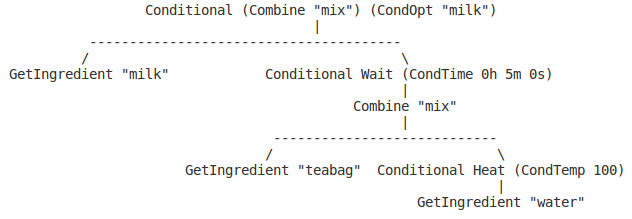
\includegraphics[width=\textwidth, keepaspectratio]{cupOfTea.png}
\centering
\caption{Cup of tea recipe printed as a tree.}
\end{figure}

One could of course use any other graphics printing package available in Haskell.

\subsection{Custom Combinators}

As mentioned previously, the combinators are highly extensible. We will now explore this
further while constructing a more complex recipe, chicken jalfrezi with rice.
For conciseness I shall omit the ingredient definitions. First of all, let's
create a marinate combinator for our chicken. This can also make use of the
fact that we may frequently want to combine many things at once.

\begin{lstlisting}
    multiCombine :: String -> Recipe -> [Recipe] -> Recipe
    multiCombine s r [] = r
    multiCombine s r rs = foldr (combine s) r rs

    marinate :: Recipe -> Recipe -> Time -> Recipe
    marinate r m t = waitFor t
        $ heatTo 4
        $ combine "cover in" r m
\end{lstlisting}

The \texttt{heatTo 4} step implies that recipe must be left to marinate in the fridge,
or somewhere else that can keep it cool. Secondly we can create a "preheat oil" combinator
for use when frying our onions and chicken.

\begin{lstlisting}
    preheatOil :: Recipe
    preheatOil = heatForM 2 oliveOil
\end{lstlisting}

Note that \texttt{heatForM} is just a variation of \texttt{heatFor} that takes time as
minutes rather than seconds for convenience. We can now start to create all the
components of our chicken jalfrezi.

\begin{lstlisting}
    spiceMix :: Recipe
    spiceMix = multiCombine "mix" cumin
        [coriander, turmeric]

    spicedChicken :: Recipe
    spicedChicken = marinate chicken
        spiceMix (minutes 10)

    cookedChicken :: Recipe
    cookedChicken = heatForM 15
        $ combine "place in" spicedChicken
        $ preheatOil

    jalfreziSauce :: Recipe
    jalfreziSauce = combine "mix" tinnedTomatoes
        $ heatForM 10
        $ combine "place in" garlic
        $ combine "place in" onion
        $ preheatOil
\end{lstlisting}

Moving onto the rice, we can abstract the notion of boiling "something" in water as we may
want to reuse this in the future, for example when cooking vegetables.

\begin{lstlisting}
    boilInWaterForM :: Time -> Recipe -> Recipe
    boilInWaterForM t r = forTime (minutes t) 
        $ combine "place in" r
        $ heatTo 100 water
\end{lstlisting}

Now we can finish by combining our chicken and sauce with a few more ingredients,
heating it for a few more minutes and then placing it on top of some boiled rice.

\begin{lstlisting}
    chickenJalfrezi :: Recipe
    chickenJalfrezi = heatForM 10
        $ multiCombine "mix" cherryTomatoes
            [garamMasala, cookedChicken, jalfreziSauce]

    jalfreziWithRice :: Recipe
    jalfreziWithRice = combine "on top" chickenJalfrezi
        $ boilInWaterForM 10 rice
\end{lstlisting}

\section{Deriving Equality}

When considering what it means for two recipes to be equal one
might consider that they must have the same ingredients
and the same actions must be performed on those ingredients,
in the same order.

\medbreak

Our recipe tree already encodes the ingredients and the actions
performed on them, they are nodes in the tree. Ordering of
actions in our tree is captured by their level in the tree.
We can see that the actions we could choose to perform first
are the leaves of the tree. If we then remove a leaf and perform
that action then the actions we can perform next are the new
leaves of the tree. This set of actions we can perform at a given time
gets smaller as we progress up to the root node of the tree where all
we can do is perform the final action. The diagram below visualises
this, albeit the number of actions would not necessarily decrease
in such a uniform fashion.

\begin{figure}[h]
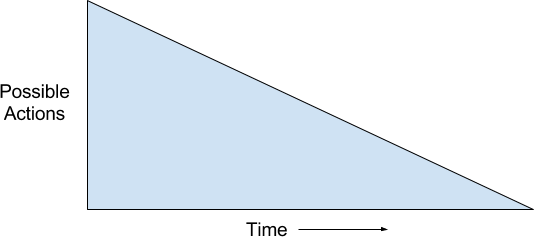
\includegraphics[width=7cm, keepaspectratio]{actionsOverTime.png}
\centering
\caption{Number of actions decrease over time.}
\end{figure}

We can use this to generate a list of all
the different orders that the actions of a recipe can be performed
in while creating the same recipe. We want a way of generating
all combinations of nodes such that nodes higher in the tree
appear after their children in the list thus preserving the
order of our actions. In other words we want a method of enumerating
all valid execution paths through our recipe.

\medbreak

This is known as topological sorting. I have implemented a
function in Haskell below which, given a recipe, returns a list
of all topological sorts of that recipe.

\begin{lstlisting}
    topologicals :: Recipe -> [[Action]]
    topologicals (Node a []) = [[a]]
    topologicals t = concat
        [map (a:) (topologicals' l) | l@(Node a _) <- ls]
        where
            topologicals' l = topologicals $ removeFrom t l
            ls = leaves t
\end{lstlisting}

This is similar to the operational semantics given by unfolding a
term to provide a list of execution paths \cite{hutton}. As an example,
consider this alternate definition for our cup of tea recipe.

\begin{lstlisting}
    cupOfTea' :: Recipe
    cupOfTea' = optional $ combine "mix" 
        ( removeAfter (minutes 5)
        $ combine "mix" teabag
        $ heatTo 100 water ) milk
\end{lstlisting}

In this version we combine our tea with milk rather than combing milk with our tea.
Printing the tree for this recipe gives a different result from our original recipe.
But fundamentally we know it to be a variation of the same recipe.

\begin{figure}[h]
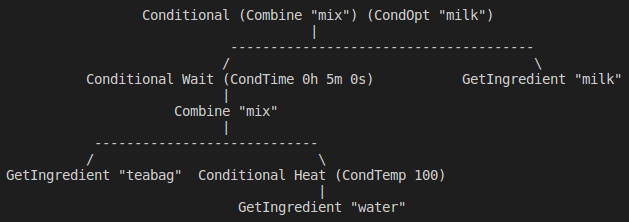
\includegraphics[width=\textwidth, keepaspectratio]{cupOfTea2.png}
\centering
\caption{Alternate cup of tea recipe printed as a tree.}
\end{figure}

In Haskell one must make their type an instance of the \texttt{Eq} typeclass in
order to make use of the \texttt{==} operator. In order to run QuickSpec on recipes
as discussed in a later section, we also need an instance of \texttt{Ord}.
This means implementing a function \texttt{compare}, which, when given two recipes,
returns an ordering for example "less than" (\texttt{LT}).

\begin{lstlisting}
    instance Ord Recipe where
        compare t1 t2 = let xs = sort $ topologicals t1
                            ys = sort $ topologicals t2
                         in compare xs ys
\end{lstlisting}

What we're doing here is taking the list of topological sorts of each recipe, sorting those
lists so that we have some consistent or and then comparing them. The \texttt{compare} function
is already implemented for lists of topological sorts as they have type \texttt{[[Action]]}
and thus they use the ordering instance already defined for Haskell lists. We do however,
need to define ordering for \texttt{Action} and all the types that \texttt{Action} uses
for example \texttt{Condition} for this to work. For this we just let GHC derive them for
us as they don't need to have any special meaning, they just need to provide a consistent
way of sorting the lists.

\medbreak

What this results in is recipes being equal if and only if their topological sorts are identical.
Recipe a will be less than recipe b if the list of recipe a's topological sorts is shorter than recipe b's.
Similarly the inverse is true of recipe a being greater than recipe b. Things become a little less
clear when the two lists are the same length. Ordering is then deferred to which lists of actions
consists of actions with lower ordering as defined by the derived ordering instance for actions.
Once again this has no actual meaning but provides the list comparison we need. With ordering defined for recipes,
defining \texttt{(==)} becomes trivial as we just check if \texttt{compare} evaluates to \texttt{EQ}.

\begin{lstlisting}
    instance {-# OVERLAPPING #-} Eq Recipe where
        (==) r1 r2 = compare r1 r2 == EQ
\end{lstlisting}

Because \texttt{Recipe = Tree Action} it naturally uses the equality instance for
\texttt{Tree} but we want to use our \texttt{compare} function which makes use of topological sorting.
That's what the "overlapping" annotation is for. Using the above definition, the expression
\texttt{cupOfTea == cupOfTea'} evaluates to \texttt{True} showing that, as desired, our two recipes are equal.

\section{Scheduling Recipes}

Now that we have a solid representation of our recipes in Haskell we can think about how
these could be scheduled.

\subsection{Modelling a Kitchen}

The first step of scheduling a recipe is to consider some representation of the
environment within which it is scheduled. Abstracting from the details we can
break a kitchen down into a set of stations for example an oven and a kettle.
We also need some sort of global observables for example, time.

\begin{lstlisting}
    data Env = Env
        { eStations :: [Station]
        , eObs      :: [IO Obs]
        }

    data Station = Station
        { stName     :: String
        , stConstrF  :: ConstraintF
        , stObs      :: [IO Obs]
        }

    type ConstraintF = Recipe -> Maybe [Process]
\end{lstlisting}

Stations consist of a name, a constraint function and a set of local observables such as temperature.
The constraint function takes a recipe and returns a list of processes required to perform that recipe.
In the event that the station cannot handle that particular recipe then \texttt{Nothing} is returned.
Observables are represented as follows. I have also provided the function that checks whether a
condition is true given a list of observables.

\begin{lstlisting}
    data Obs = ObsTemp Int
             | ObsTime Time
             | ObsOpt String Bool

    evalCond :: Condition -> [Obs] -> Bool
    evalCond (CondTime t) os = case [o | o@(ObsTime _) <- os] of
        [] -> False
        (ObsTime t' : _) -> t == t'
    evalCond (CondTemp t) os = case [o | o@(ObsTemp _) <- os] of
        [] -> False
        (ObsTemp t' : _) -> t == t'
    evalCond (CondOpt s) os = case [o | o@(ObsOpt s' _) <- os, s == s'] of
        [] -> False
        (ObsOpt _ b : _) -> b
    evalCond c os = getAll $ foldCond (\c -> All $ evalCond c os) c
\end{lstlisting}

A process is an intermediate translation of our recipes. One might say it's our sort of assembly
language, sitting between our high level combinators and some device specific instructions that the
developer of a robot chef might write.

\begin{lstlisting}
    data Process =
        Input
        | Output
        | Preheat Int
        | DoNothing
        | PCombine String
        | EvalCond Condition
        | MeasureOut Measurement
\end{lstlisting}

Most of these are self explanatory, \texttt{PCombine} and \texttt{MeasureOut} are just renamings of
the actions \texttt{Combine} and \texttt{Measure}. \texttt{EvalCond} is inserted after \texttt{Input}
which when interpreted will check the condition, if true then skip to \texttt{Output} else it will
run all processes up until \texttt{Output} before jumping back to the condition again. As an example,
here is part of our cup of tea recipe translated into a list of processes.

\begin{lstlisting}
    Conditional (CondTemp 100) Heat ->
        [Input, EvalCond (CondTemp 100), Output]
\end{lstlisting}

The water is put into the kettle which then heats it until the temperature is 100 degrees
before the water is taken out. You might be wondering why there is no "heat" process.
That's because something is heated as a side effect of being placed in a device which becomes hot
rather than as an explicit action of that device. Device specific details such as the kettle turning
on when the water is added or turning off on output is not covered here as these details can
be abstracted away being \texttt{Input} and \texttt{Output}.

\medbreak

Now let's consider what stations we require to make our cup of tea. At the most basic level
we need a kettle and a chef. For conciseness I shall only discuss the kettle.

\begin{lstlisting}
    kettle :: Station
    kettle = let kettleConstr r@(Node a ts)
                    | r == heatTo 100 (ingredient "water") = Just [Input, Output]
                    | otherwise = case a of
                        Transaction a -> kettleConstr $ popT r
                        _ -> Nothing
                 kettleTemp = return $ ObsTemp 100
              in Station "kettle" kettleConstr [kettleTemp]
\end{lstlisting}

Here we're creating a station with a name of "kettle", creating the constraint function
and also providing a temperature observable. We have no actual kettle to retrieve the temperature
from so for now we are just providing a constant temperature of 100 degrees. The constraint function
simply checks if the recipe passed is "boiling water" or "boiling water" wrapped in a transaction (Section 4.5),
returning Nothing if it's not.

\medbreak

We can now speicfy our environment as follows. I have added an extra uneeded station, a toaster,
to demonstrate that it remains unused when scheduling making a cup of tea.

\begin{lstlisting}
    env :: Env
    env = Env { eStations = [kettle, chef, toaster]
              , eObs = [ getTime
                       , return $ ObsOpt "milk" True ] }
\end{lstlisting}

The function \texttt{getTime} simply returns the UTC time converted to \texttt{ObsTime}.
We then need to provide a value for our optional "add milk" step. The observables are
wrapped in IO meaning they can come from external sources for example, the command line
if we so desired.

\subsection{Scheduling Methods}

Now that we have a model of a cooking environment we need to choose a method for scheduling the recipes.
Scheduling is in itself a complex problem and therefore the solution used for this project is by
now means suggested as a well refined solution but merely a demonstration of using the recipe system
for a more concrete purpose.

\subsubsection{Linear Programming}
The first consideration was linear programming (LP). LP works by taking a linear function, called
the objective function, which is minimised or maximised according to a set of linear constraints.
For our recipes the objective function would be the end time of the final step which we would then
want to minimise in order to make the recipe as efficient as possible. We then might consider the
following constraints.

\[ end_r = start_r + dur_r \quad \forall r \]

\[ start_r \geq end_d \quad \forall d,r \quad | \quad d \in dependencies(r) \]

That is the end time of each recipe is equal to its start time plus its duration and a recipe
must start at or after the end time of its dependencies.

The problem arose with choosing which station to schedule each action on. For any action we
have a set of stations that can perform that action. We can then expand our first constraint
to handle this.

\[ end_{r_s} = start_{r_s} + dur_{r_s} \quad \forall r,s \quad | \quad s \in validStations(r) \]

But we only want one of the valid stations to be selected which leaves us with the problem
of modelling logical OR in this context. One potential way is to use a set of binary variables
as follows.

\[ end_r = \sum (end_{r_s} * bin_{r_s}) \quad \forall r,s \quad | \quad s \in validStations(r) \]

\[ \sum_{s}^{validStations(r)} end_{r_s} = 1 \quad \forall r \]

The issue with the above is that it involves the multiplication of two variables. As such this
is no longer a linear constraint. A long time was spent considering whether or not our recipes
could in fact be expressed as linear systems. After reformulating the problem several times
and not finding a solution I decided to move on from linear programming and find something else.

\subsubsection{Bin Packing}

Bin packing is a much more general optimisation problem. It is the problem of packing a number
of objects with fixed dimensions into a number of bins of fixed dimensions such that the number
of bins is minimised. This problem as it is doesn't bare much resemblance to our recipes however,
adjusting the problem as follows provides something more useful.

\medbreak

Given a number of objects of fixed height and a number of bins of infinite height where each
bin can only hold certain types of object. Pack the objects into the bins such that the
height of the tallest stack is minimised and a set of constraints regarding order of
objects is met. We can model our stations as a stack of actions which they must perform,
these are our bins. Our objects are either the station performing one of our actions
or being idle for a certain time. We can then say that the height an action begins on
the stack must be greater than or equal to the height that its dependencies end on their
respective stacks.

\medbreak

As an abstract example, imagine a recipe, r1, which has sub-recipes: r2, r3 and r4. All the
recipes must be scheduled on station 2, except r3 which must be scheduled on station 1.
Below is a diagram showing r1 and a potential stack setup.

\begin{figure}[h]
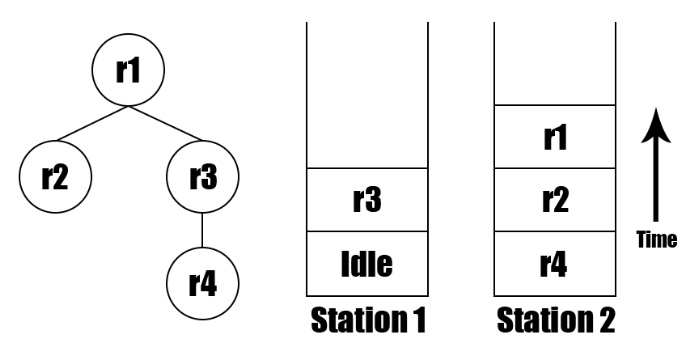
\includegraphics[width=10cm, keepaspectratio]{stacks.png}
\centering
\caption{Recipe tree and stack schedule for r1.}
\end{figure}

\subsection{Optimisations and Heuristics}

Now that we have a way to translate our recipes into a form of schedule we need to consider
optimisations we can apply during the scheduling process. As mentioned in the introduction,
you have no doubt done this while cooking at home. In the case of making a cup of tea you
may start the kettle boiling before you get the milk out of the fridge. That way, you and
the kettle are working in parallel and thus saving time.

\medbreak

Heuristics are "rules of thumb" that are applied to a problem solver in order to guide it
in the decision making process. An everyday example might be preferring motorways over country roads
when planning a journey; they have a higher speed limit and traffic capacity thus making
them a faster route in the general case. There are two decisions we can apply heuristics to
when scheduling recipes. The first is which leaf of the recipe tree to schedule first.
Referring back to the section on topological sorting (Section 3), the leaves of the tree at a given time
are comprise the set of actions we can choose to perform next. The second decision is which
of the available stations to schedule this action on.

\subsubsection{Leaf Choice Heuristics}

The first heuristic used in leaf choice is "shortest task first". This may seem counter intuitive however,
if we think about the way in which recipes are typically structured, it makes sense. It is frequent
to have a small task such as "get water" followed by a longer task performed by another station
for example "boil water". Let's say that "get milk" was a long task to complete. It would make more
sense to do the short "get water" task first, start the kettle boiling, then use that time to
"get milk". If we "get milk" first then we're performing a long task, meanwhile the kettle is idle
waiting for some water.

\medbreak

The second heuristic is applied in the event that multiple leaves contain a task of the shortest length.
It is based on the same principle as above, that if we have short task such as "get water" followed
by a lengthy task such as "boil water" we want to "get water" as soon as possible so that the kettle
can be boiling while we do the other tasks. This is formalised as "longest branch first". In the
event that there are multiple "shortest tasks" then the task on the longest branch will be chosen
to try and ensure that if we have a long task that depends on a short task, it will be started
as soon as possible.

\subsubsection{Stack Choice Heuristics}

Now that we have selected which leaf to schedule, we need to choose which station to schedule it on.
In many cases this is a simple task as many actions can only be performed by one station. In the event
that multiple stations can be used then we use three heuristics to choose, each shortening the list of
potential stations.

\medbreak

The first is to pick whichever station is in least demand. This is done by scanning through all unscheduled
actions and calculating their time divided by the number of stations that action could be performed on.
For example if an action a had a time of 10 and could be performed on either of 2 stations then the demand
that a would create for each station would be 5. The reason for this heuristic is rather intuitive. If we
have a choice between a station which a lot of other actions need and a relatively uneeded station, we should
choose the uneeded station to reduce the load on the high demand station. This heuristic could obviously
be inverted if the goal was to minimise stations used rather than time taken.

\medbreak

The second heuristic is "least idle time". One's first thought might be to add the action to the emptiest
stack however, in the event that the action is waiting on a long dependency, it could cause lots of idle
time to be added to an otherwise empty stack. Therefore we choose the stack which allows the action to be
started closest to the end time of its dependencies which may mean placing it on a fuller stack rather than
an emptier one. We also might consider that choosing an a stack with "high demand" could be worth it if
it avoids a significant amount of idle time. To model this we implement these two heuristics as one by
simply adding the idle time and demand of a station together. We can then choose or choose from the
station(s) with the lowest idle time and demand.

\medbreak

It is unlikely that the first two heuristics didn't filter the potential stations down to one, but if they
didn't then we select the stack that is least full. Providing there are no caveats like idle time, as mentioned
above, then placing an action on an emptier stack should result in a shorter overall time in most cases.

\subsection{Implementation}

In the interest of space, I shalln't go into the details of the code here as there is quite a lot of it
However, below is some pseudo-code to demonstrate the general flow of the scheduling functions.

\begin{lstlisting}
    data Task = Active Label | Idle Time

    type Stack = [Task]

    type Schedule = Map StName Stack

    schedule :: Recipe -> Env -> Schedule
    schedule r env = do
        tree = labelRecipe r
        schedule' env tree tree emptySch
        where
            schedule' env fullTree tree sch = do
                l = chooseLeaf tree
                st = chooseStation fullTree l env sch
                stack = lookup st sch
                stack' = Active l : stack
                newSch = insert st stack' sch
                if l == root fullTree
                    then
                        newSch
                    else
                        tree' = removeFrom tree l
                        schedule' env fullTree tree' newSch
\end{lstlisting}

The main function \texttt{schedule} takes a recipe and an environment then returns a schedule.
It first labels the recipe, this is to avoid issues with a set of actions appearing on multiple
branches. It then passes the environment, two copies of the recipe tree and an empty initial
schedule to the sub-routine \texttt{schedule'}. The reason for passing two copies of the tree
is that one is maintained as the full tree in order to maintain access to the children of the
node we are scheduling even after those child nodes have been scheduled and removed from the other
tree. The functions \texttt{chooseLeaf} and \texttt{chooseStation} apply the various heuristics
and return the best leaf and best station respectively. Next we add the leaf to the stack of
the chosen station and update the schedule. We then check to see if the node we just
scheduled is the root of the tree, if it is, then we have finished and can return our new schedule
otherwise we pass our new schedule and updated tree to the next iteration of \texttt{schedule'}.

\medbreak

The function \texttt{scheduleAndPrint} schedules a recipe on a given environment
and prints the result in a more readable way, showing each action as a step rather
than a collection of the more low level processes. Below is the result of running
\texttt{scheduleAndPrint} on our cup of tea and the environment created above.

\begin{lstlisting}
> scheduleAndPrint cupOfTea env = 

chef:
0h 0m 0s: 3) Get water
0h 0m 10s: 2) Get teabag
0h 0m 20s: 1) Get milk
0h 0m 30s: Idle: 0h 3m 0s
0h 3m 30s: 5) mix (2) and (4)
0h 3m 40s: 6) Wait for 0h 5m 0s
0h 8m 40s: 7) mix (1) and (6) (optional)

kettle:
0h 0m 0s: Idle: 0h 0m 10s
0h 0m 10s: 4) Heat (3) until temperature 100

toaster:
\end{lstlisting}

As you can see the scheduling function tells the chef to get the water first so that the
kettle can start boiling it as soon as possible. After 10 seconds the kettle can start
boiling the water, meanwhile the chef acquires the other ingredients before becoming idle
until the kettle has finished. Once the water is boiled the chef adds the teabag before
waiting for 5 minutes. After that they optionally add milk. Meanwhile our uneeded toaster
does nothing. While this scheduling function seems effective, it is also rather inefficient.
When running it on larger recipes like our chicken jalfrezi, which contains over 30 steps,
it runs for a long time before running out of memory. As mentioned before, the scheduling
function isn't the focus of the project and as such not a lot of time was spent on it.

\subsection{Transactions}

This method of scheduling seems to work however, there is one problem that arises from us
reordering steps in order to optimise them. Consider the following recipe for tea and buttered toast,
for conciseness I have omitted the ingredient definitions.

\begin{lstlisting}
    cupOfTea :: Recipe
    cupOfTea = optional $ combine "mix" milk
        $ waitFor (minutes 5)
        $ combine "mix" teabag
        $ heatTo 100 water

    butteredToast :: Recipe
    butteredToast = combine "spread" butter
        $ heatFor (minutes 3) bread

    teaWithToast :: Recipe
    teaWithToast = combine "place next to"
        butteredToast
        cupOfTea
\end{lstlisting}

It could be the case that, when scheduling, first the bread is toasting, then the cup of tea is
made, then the butter is added to the toast. The problem with this is that by the time we come
to spread the butter on the toast, it has gone cold. We need some way to ensure that the butter
is added immediately after the toast is finished. To do this we have a new combinator called
\texttt{Transaction} which wraps any other action. This can then be interpretted by the scheduling
function to mean that the action which it wraps and it's immediate children should be scheduled
together meaning that no other actions can end up in between. Our buttered toast recipe is now
as follows.

\begin{lstlisting}
    butteredToast :: Recipe
    butteredToast = transaction
        $ combine "spread" butter
        $ heatFor (minutes 3) bread
\end{lstlisting}

\section{Recipe Properties}

In this section we will explore recipes across various semantic domains and how this can
help us to create new recipes.

\subsection{Folding Over Recipes}

One function that is particularly useful in exploring semantics is \texttt{fold}.
Folding is the process of taking some whole made up of parts and creating a single
value from it. For example folding texttt{(+)} over a list of numbers \texttt{[1,2,3]}
returns 6. We can use folding to create denotational semantics for our recipes \cite{hutton}.
Denotational semantics involves terms being evaluated via a mapping to a value in a certain
semantic domain. There are multiple semantic domains of interest in recipes hence the choice
of a deep embedding (Section 1.3). Abstracting the traversal of the recipe from the
semantic mapping functions, into a fold function results in conciser definitions and
less repetition.

\begin{lstlisting}
    foldRecipe :: Monoid a => (Action -> a) -> Recipe -> a
    foldRecipe f (Node a ts) =
        let vs = map (foldRecipe f) ts
         in f a `mappend` (mconcat vs)
\end{lstlisting}

Now that we have defined folding over recipes, we can take any function which maps actions
to some value and use it to evaluate our recipe. The one caveat is that the values must form
a monoid. This simply means that the values should have some "empty" value and that there should
be some natural way of appending them. As an example the \texttt{Monoid} instance of
\texttt{Time} is given below.

\begin{lstlisting}
    instance Monoid Time where
        mempty = 0
        mappend = (+)
\end{lstlisting}

\subsection{Time}

An important semantic domain for recipes is time. In order to calculate the
time of a recipe using \texttt{foldRecipe} we first need a function of type \texttt{Action -> Time}.

\begin{lstlisting}
    timeAction :: Action -> Time
    timeAction (GetIngredient _) = 10
    timeAction Heat = 0
    timeAction (HeatAt t) = preheatTime t
    timeAction Wait = 0
    timeAction (Combine _) = 10
    timeAction (Conditional _ c) = foldCond f c
        where
            f (CondTime t) = t
            f (CondTemp t) = tempToTime t
            f (CondOpt s) = 0
    timeAction (Transaction a) = timeAction a
    timeAction (Measure m) = 10
\end{lstlisting}

These times are just intended to be estimates, note that most of the "time" is contained within
conditionals. This is intentional as most of the duration of a recipe is made up of performing an
action for a given time rather than actions that have a set time. A more complex function might
also take into account which station each action is scheduled on. The only other point of note
here is \texttt{foldCond}. This function allows us to abstract the details of "and" and "or"
conditions to a more general case as follows.

\begin{lstlisting}
    foldCond :: (Ord a, Monoid a) => (Condition -> a) -> Condition -> a
    foldCond f (c `AND` c') = (foldCond f c) `mappend` (foldCond f c')
    foldCond f (c `OR` c')  = max (foldCond f c) (foldCond f c')
    foldCond f c            = f c
\end{lstlisting}

If the condition we are handling is logical and over two conditions then we can simply apply our function
to each of the sub-conditions and join the results, hence the requirement that the value we're
creating have a monoid instance. In the that event we're dealing with the logical or of two conditions then
we apply our function to each of the sub-conditions as before, except this time we take the largest value.
This provides us with a "worst case scenario" as it would take whichever condition would take the longest
duration to be met. This works in other semantic domains too. Imagine we added a condition of mass and thus
extracted the measurement from our \texttt{Measure} combinator (Section 5.3). If we calculated the cost of a recipe, as we shall
do in the next section, we would need to quantify the ingredients. Using \texttt{foldCond} on logical or over two
conditions in the domain of mass would provide us with the largest mass possible leading to the highest price and
once again the "worst case scenario". Our use of \texttt{max} also holds when evaluating conditions to boolean values
as \texttt{max True False = True} thus holding the meaning of logical or.

\medbreak

We can now define our function \texttt{time} for a recipe as follows.

\begin{lstlisting}
    time :: Recipe -> Time
    time = foldRecipe timeAction
\end{lstlisting}

We can also define a function \texttt{schLength} which tells us the length of a schedule.

\begin{lstlisting}
    schLength :: Schedule -> Recipe -> Time
    schLength sch r =
        let rMap = mkLabelMap $ labelRecipeR r
            stacks = Map.elems sch
            ts = map (\s -> stackHeight s rMap) stacks
         in maximum ts
\end{lstlisting}

One of the great things about Haskell is that it allows us to keep the recipe labelling
functions pure. As such we can recreate the map of labels to recipes that was used in
scheduling at any point and know it will be the same; we need not worry that some side
effect has caused it to be different.

\medbreak

If we run the above functions on our cup of tea then we see that our scheduling has
saved us 20 seconds off the estimated time by parallelising certain steps. Naturally
this benefit would potentially be much larger for a recipe with a larger number of steps.

\begin{lstlisting}
    > time cupOfTea = 0h 9m 10s

    > schLength (scheduleRecipe cupOfTea env) cupOfTea = 0h 8m 50s
\end{lstlisting}

\subsection{Price}

Another semantic domain to consider for recipes is their price. For this we
need to quantify our ingredients with the \texttt{Measure} combinator.

\begin{lstlisting}
    data Measurement = Count Int | Grams Int | Milliletres Int

    measure :: Measurement -> Recipe -> Recipe
    measure m r = Node (Measure m) [r]
\end{lstlisting}

Below is our cup of tea recipe, updated with quantified ingredients.

\begin{lstlisting}
    cupOfTeaQ :: Recipe
    cupOfTeaQ = optional "milk"
        $ combine "mix" (measure (Milliletres 10) milk)
        $ waitFor (minutes 5)
        $ combine "mix" (measure (Count 1) teabag)
        $ heatTo 100
        $ measure (Milliletres 300) water
\end{lstlisting}

We now need some representation of the price of the individual ingredients.
Below is an implementation of a \texttt{PriceList} which itself is based on
a more generic \texttt{PropertyList}.

\begin{lstlisting}
    type PropertyList v = [(String, v)]

    type PriceList = PropertyList (Price, Measurement)
\end{lstlisting}

Finally we need to get a list of our quantified ingredients and check them
against the price list.

\begin{lstlisting}
    evalPropsQ :: (Integral v, Monoid v) => PropertyList (v, Measurement)
                    -> [(String, Measurement)] -> v
    evalPropsQ ps xs = mconcat $ map evalPropsQ' xs
        where
            evalPropsQ' (s,m) = case lookup s ps of
                Nothing -> mempty
                Just (v,m') -> applyQuant m (v,m')
\end{lstlisting}

The function \texttt{evalPropsQ} takes a list of properties, that have a \texttt{Measurement}
component, and a list of \texttt{String} keys that also have a \texttt{Measurement}.
We then lookup each key in our list, use \texttt{applyQuant} which calculates the ratio
of measurements returning the actual price (or other value) for our quantity, and finally
join the results together making use of our value's monoid instance.

\medbreak

We can now define \texttt{price} for our recipes. Note \texttt{ingredientsQ} takes a recipe
and returns a list of ingredient names paired with their measurements.

\begin{lstlisting}
    price :: PriceList -> Recipe -> Price
    price ps r = evalPropsQ ps (ingredientsQ r)
\end{lstlisting}

Returning to our quantified cup of tea, we get the following.

\begin{lstlisting}
    priceList :: PriceList
    priceList = [ ("teabag", (639, Count 240))
                , ("milk", (70, Milliletres 1000))
                , ("sugar", (69, Grams 1000))
                , ("water", (0, Milliletres 1)) ]

    > price priceList cupOfTeaQ = (*@{\pounds}@*)0.04
\end{lstlisting}

\subsection{QuickSpec}

QuickSpec \cite{quickspec, quickspec2} is a Haskell library for automatically generating
laws about your program. In order to do this, QuickSpec requires a way of generating
random values of the relevant type. We can provide this by making our recipe type
an instance of the \texttt{Arbitrary} typeclass.

\begin{lstlisting}
    instance {-# OVERLAPPING #-} Arbitrary Recipe where
        arbitrary = sized $ \n -> do
            if n <= 5 then
                genRecipe n
            else
                resize 5 arbitrary

    genRecipe :: Int -> Gen Recipe
    genRecipe n =
        let un = resize (n-1) arbitrary
            bin = resize (n `div` 2) arbitrary
        in if n == 0 then
                genIng
            else
                oneof [genUnRec un, genBinRec bin bin]

    genIng :: Gen Recipe
    genIng = liftM (ingredient . show)
        (choose (1, 100) :: Gen Int)

    genUnRec :: Gen Recipe -> Gen Recipe
    genUnRec un = oneof
        [ liftM heat un
        , liftM2 heatAt genTemp un
        , liftM wait un
        , liftM2 addCondition arbitrary un
        , liftM transaction un
        , liftM2 measure arbitrary un ]

    genBinRec :: Gen Recipe -> Gen Recipe -> Gen Recipe
    genBinRec r1 r2 = liftM3 combine genMethod r1 r2
\end{lstlisting}

The first point of note is that our recipes are generated as sized values meaning
that they have a number of sub-recipes. If a recipe is size 0 then we should generate
an ingredient. Random ingredients are just provided as a random number between 1 and 100.
If the size of the recipe is greater than 0 then we can either generate a unary recipe
or a binary recipe. This refers to how many children the recipe should have. The only
valid binary recipe we have is combine, the rest are all unary as they only apply to
one sub-recipe. Instances of \texttt{Arbitrary} are also required for all the other types
needed to make recipes such as \texttt{Time} and \texttt{Measurement}. In the interest
of space I shalln't go into them here, they are relatively straightforward compared to
the above. We also limit the size to a maximum of 5 due to how computationally expensive
it is to compare larger recipes.

\medbreak

The other interesting definition is that for \texttt{Condition} as conditions don't
have a natural ordering instance. Instead, QuickSpec allows us to test for observational
equality. That is we must specify a function \texttt{observe test a} for which the
following property holds: \textit{two values x and y are considered equal,
if for many random values of type test, observe test x == observe test y} \cite{quickspec-docs}.

\begin{lstlisting}
    instance Arbitrary Obs where
        arbitrary = oneof
            [ liftM ObsTemp genTemp
            , liftM ObsTime arbitrary
            , liftM2 ObsOpt (liftM show
                (choose (1, 10) :: Gen Int)) arbitrary ]

    instance Observe [Obs] Bool Condition where
        observe obs c = evalCond c obs
\end{lstlisting}

Below we are generating random lists of our \texttt{Obs} type and evaluating our
condition against them (Section 4.1). Now that we have all of our instances,
we can pass our recipe functions to QuickSpec and see what laws it finds.

\subsection{Generating Recipes}

While QuickSpec deals with recipes generated arbitrarily, we could also
consider how we might generate recipes in a more structured way. This could
then be combined with the semantics discussed above to work out the cheapest
or most time efficient meals that meet certain criteria. If we want a dish
to have certain properties then we first need to create a list of our
available ingredients and map them to their properties. As a simple
example, here is a list of ingredients given a property called
\texttt{FoodType} which simply lables whether the ingredient is a meat
or a vegetable.

\begin{lstlisting}
    data FoodType = Meat | Veg

    ingList :: PropertyList FoodType
    ingList = [ ("chicken breast", Meat)
              , ("beef sirloin", Meat)
              , ("lamb chop", Meat)
              , ("broccoli", Veg)
              , ("carrot", Veg)
              , ("cauliflower", Veg)
              , ("green beans", Veg)
              , ("green cabbage", Veg)
              , ("potato", Veg) ]
\end{lstlisting}

We also need to know how to cook each ingredient so we will create another
list which maps the ingredient to a recipe. There are, of course, many different
ways that one could cook each ingredient and this could easily be adapted to
map ingredients to a list of recipes. For simplicity though, we shall just
stick with one.

\begin{lstlisting}
    recList :: PropertyList Recipe
    recList = [ ("chicken breast", heatAtForM 200 40 $ ingredient "chicken breast")
              , ("beef sirloin", heatAtForM 200 20 $ ingredient "beef sirloin")
              , ("lamb chop", heatAtForM 200 17 $ ingredient "lamb chop")
              , ("broccoli", boilInWaterForM 5 $ ingredient "broccoli")
              , ("carrot", boilInWaterForM 5 $ ingredient "carrot")
              , ("cauliflower", boilInWaterForM 7 $ ingredient "cauliflower")
              , ("green beans", boilInWaterForM 5 $ ingredient "green beans")
              , ("green cabbage", boilInWaterForM 5 $ ingredient "green cabbage") ]
\end{lstlisting}

Now we need some structured way of selecting ingredients and then combining
them. We call this a "cuisine". The type of cuisine that we are making provides
the structure that the ingredients will be placed into. To demonstrate this
concept we will use the very simple and traditional "meat and two veg".

\begin{lstlisting}
    type Cuisine a = PropertyList a -> Recipe

    meatTwoVeg :: Cuisine (FoodType, Recipe)
    meatTwoVeg ps =
        let meats = filter (\(_,p) -> fst p == Meat) ps
            vegs = filter (\(_,p) -> fst p == Veg) ps
            parts = map (\(_,p) -> snd p)
                    $ head meats : take 2 vegs
        in foldr1 (combine "next to") parts
\end{lstlisting}

Here we are simply seleting a meat and two vegetables, taking their
recipes from the list and then combining them in an appropriate way.
Running this example we get the following recipe tree.

\begin{figure}[h]
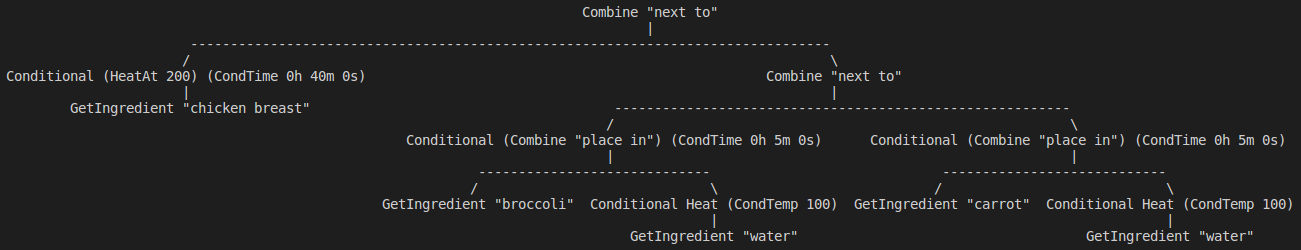
\includegraphics[width=\textwidth, keepaspectratio]{meatTwoVeg.png}
\centering
\caption{Recipe tree for generated recipe example.}
\end{figure}

This is of course a very simple example, one could imagine modelling much more complex
cuisines with this method, maybe even handling the cooking methods for each type of
ingredient in the cuisine function itself rather than having a list. This could also
be interfaced with some sort of machine learning algorithm which has processed
many recipes in a given cuisine to find common flavour combinations.

\subsection{Improving Recipes}

We have looked into how we can generate new recipes but what about improving recipes
that already exist, or indeed that we have generated? One of the easiest ways to
improve a dish is to ensure it has been properly seasoned. Typically people think
of salt and pepper when seasoning but there is actually a seasoning triangle \cite{seasoning},
consisting of salt, sugar (sweetness) and acid. A dish will taste better if these
flavours are all in balance.

\medbreak

Let's start by modelling these seasonings as a data type. We can also model a
"flavour profile" as a list of seasonings paired with the frequency they appear
in our recipe.

\begin{lstlisting}
    data Seasoning = Salt | Sweet | Acid
        deriving (Eq, Ord, Show)

    type Profile = [(Seasoning, Int)]
\end{lstlisting}

Next we can write a function \texttt{profile} that, given a list of seasonings,
turns them into a flavour profile.

\begin{lstlisting}
    profile :: [Seasoning] -> Profile
    profile [] = [(Salt, 0), (Sweet, 0), (Acid, 0)]
    profile (s:ss) =
        let m = profile ss
            i = fromJust $ lookup s m
        in insert s (i+1) m
\end{lstlisting}

Finally we can write a function \texttt{balance} which, given a recipe and
a mapping from ingredients to the seasoning that they bring to a dish,
profiles the seasonings it contains before suggesting what needs to be done
to balance them. If there are no seasonings at all, it will suggest we add
one of everything. On the other hand, if the seasonings are out of balance,
it will suggest the amount of each type of seasoning that is required
to balance the dish.

\begin{lstlisting}
    balance :: Recipe -> PropertyList Seasoning -> [(Seasoning, Int)]
    balance r ss =
        let is = ingredients r
            flavours = catMaybes $ map (\i -> lookup i ss) ings
            p = profile flavours
            (_,maxI) = maximumBy (\(_,i) (_,i') -> compare i i')
        in case p of
                [(Salt, 0), (Sweet, 0), (Acid, 0)] -> map (\(s,_) -> (s,1)) p
                _ -> [(s, maxI - i) | (s,i) <- p]
\end{lstlisting}

This could be combined with the recipe generation functions from the previous
section to actually suggest which ingredients could be added to provide
each seasoning. To add acid in Thai cuisine, one might add lime juice whereas
in Italian cuisine, red wine might be more appropriate.

\medbreak

As an example, let's consider the following, most basic of recipes, an avocado.
Avocado is often eaten on its own and has a slightly sweet, creamy flavour.
Passing this to our \texttt{balance} function we get the following.

\begin{lstlisting}
    seasonings :: PropertyList Seasoning
    seasonings = [ ("avocado", Sweet)
                 , ("salt", Salt)
                 , ("lime juice", Acid) ]

    > balance (ingredient "avocado") seasonings = [(Salt,1),(Sweet,0),(Acid,1)]
\end{lstlisting}

As you can see, we need to add some salt and some acid to our avocado in order
to balance the flavours. Adding some salt and a sequeeze of lime juice
as follows puts our flavours in balance. This is actually a basic version
of the popular dip, guacamole.

\begin{lstlisting}
    guacamole :: Recipe
    guacamole = multiCombine "mix" avocado
        [salt, limeJuice]

    > balance guacamole seasonings = [(Salt,0),(Sweet,0),(Acid,0)]
\end{lstlisting}

\section{Development Process}

\subsection{Project Management}

The project has been managed using the scrum development method with the time
between supervisor meetings actings as the sprints, typically two weeks in length.
This allowed lots of flexibility regarding the prioritisation of project
components and the length of time spent on them. Due to the research nature
of the project it wasn't clear from the outset exactly which parts would take the
longest or be the most challenging. An example of this is that
quite a significant amount of time was spent in the first part of the project
considering various semantics for recipes before other parts of the language
were started. In the second part of the project a lot of time was spent
with scheduling recipes. Trying to express the constraints in linear form
was a huge challenge and in the end it seems as though it wasn't actually possible
hence the move to bin packing.

\medbreak

Throughout the project, a Trello board was used to keep track of tasks
and prioritise them appropriately. The files for the project were stored
on GitLab providing version control and backups. Furthermore, GitLab's
continuous integration (CI) servers were used to compile the code and run
some examples to ensure any issues were found as soon as possible.

\subsection{Evaluation and Testing}

This section discusses the methods used to evaluate and test our
combinators. There are of course more features that could be
added which will be discussed in Section 7.2.

\subsubsection{QuickCheck}

QuickCheck \cite{quickcheck} is a library for the automated testing of Haskell
programs. The programmer specifies laws that must hold about their program
and QuickCheck generates random test cases to check whether or not the
law holds. A simple example would be to check that reversing a list
twice gives you the same list you started with.

\medbreak

For our recipes, we already have various laws that were discovered by QuickSpec
(Section 5.4). We can get QuickCheck to test these so that if we ever make
a change that breaks these laws, it is detected and we can check whether that
result was desired or not. This helps us to reason about what our code is actually
doing and thus have confidence of its correctness.

\medbreak

% Example of converting quickspec law into quickcheck test

\subsubsection{Test Recipes}

While QuickCheck is great for verifying the correctness of our code, it does
not measure the conciseness or expressiveness of our combinators. To do this
we have used various test recipes, as used throughout this report. Below
is a table detailing what each test recipe was used for specifically,
naturally all recipes test for conciseness.

\begin{figure}[h]
\begin{tabular}{ |p{35mm}|p{\textwidth - 40mm}| }
    \hline
    \texttt{cupOfTea} & Basic recipe. \\
    \hline
    \texttt{cupOfTea'} & Modified \texttt{cupOfTea}, used to test equality. \\
    \hline
    \texttt{cupOfTeaQ} & Quantified \texttt{cupOfTea}, used to test the \texttt{Measure} combinator. \\
    \hline
    \texttt{butteredToast} & Used to test the \texttt{Transaction} combinator. \\
    \hline
    \texttt{jalfreziWithRice} & Much longer and more complex recipe, uses
        all the combinators except \texttt{Measure} and \texttt{Transaction}. \\
    \hline
\end{tabular}
\caption{Table of test recipes and their descriptions.}
\end{figure}

\section{Summary}

\subsection{Contributions}

While DSLs are a widely explored field, nothing along the lines of a recipe DSL
currently exists. My contributions to filling this gap are the following:

\begin{itemize}
    \item A small set of extensible combinators that can be used to describe a wide variety of recipes (Section 2).

    \item Interpretations of recipes specified using these combinators within various semantic domains (Section 5).

    \item A concrete implementation in the form of stations in an environment (Section 4).

    \item A demonstration of how operational semantics (topological sorting) can be used in
    scheduling to optimise a recipe via parallelisation (Sections 3 \& 4).

    \item Mapping of various properties to recipes potentially leading to the ability
    to suggest improvements (Sections 5.5 \& 5.6).

    \item Exploration into how, given a certain model (cuisine), one can write functions that
    generate recipes (Section 5.5).
\end{itemize}

Due to the novel nature of this project there are no doubt other avenues to explore and
room to further explore those mentioned. The first stage of the project was to describe
and display recipes. We then proceeded by defining their semantics across various domains
before finally exploring applications for these semantics. This is illustrated by the
three levels of the graph below.

\begin{figure}[h]
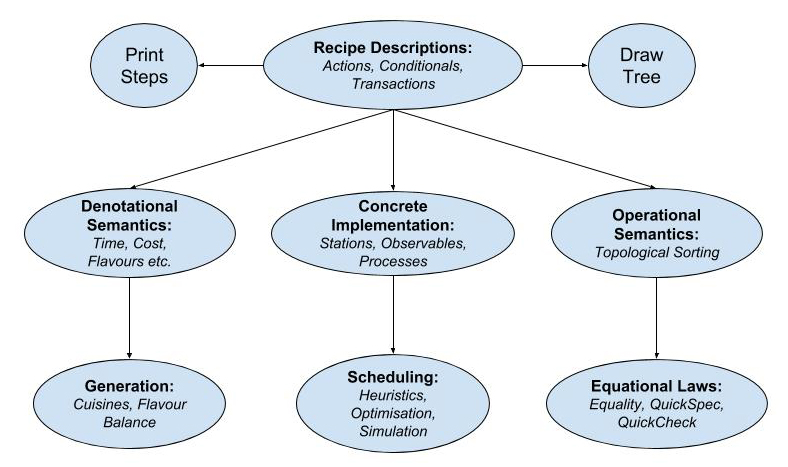
\includegraphics[width=\textwidth, keepaspectratio]{project.jpg}
\centering
\caption{Diagram displaying overall project structure.}
\end{figure}

\subsection{Future Work}

As mentioned above, there does not currently exist much, if any, work in the area of
a recipe DSL and as such there is huge scope for future work. More work is needed
to perfect and further refine the combinators. There is currently no way to
"remove" a recipe from another recipe for example removing the teabag from our cup of tea.
An unsafe version of this may just presume that way was added can in fact be removed
and that it was even added in the first place however, creating a sensible remove
combinator would no doubt require more thought.

\medbreak

A further consideration, briefly mentioned previously, is that the \texttt{Measurement}
passed to the \texttt{Measure} action should potentially be extracted into a condition.
This would allow the modelling of a "reduceBy" combinator that could be implemented as
something along the lines of the following.

\begin{lstlisting}
    reduceBy r t m = addCondition (CondMeasure m) (heatAt t r)
\end{lstlisting}

In other words: "heat the given recipe at the given temperature until it has reduced by the given measurement".

\medbreak

There is also one rather difficult issue of handling recipes that have multiple
outputs. For example let's say we roasted some meat and then wanted to take out the
meat juices to make gravy but also do something with the meat. This completely breaks
our tree structure as we would have the roast meat node branching up into two nodes,
roasted meat and meat juices. This is closely related to the "remove" problem.

\medbreak

It goes without saying that further optimisations and research could be done into the
scheduling part of this project; scheduling is, itself, a huge area of research.
The scheduling solutions expressed above were mainly to demonstrate a use of
the operational semantics of recipes.

\medbreak

Our model of a cooking environment was rather simple and didn't consider any requirement
of transferring recipes between stations. For example, once something has been heated
by an oven, it is then immediately available to any other station that needs to perform
an action on it regardless of whether a chef is available to take it out of the oven or not.

\medbreak

There is also the task of translating our processes to actual instructions specific to a certain
robot. It would be interesting to see what sort of issues would arise from this as they could then
be used to direct attention to which areas of the project are most in need of further development.

\subsection{Reflections}

Being a research oriented project this was certainly different from anything I'd ever done before.
Throughout the project there were times when I noticed that I was focusing too much on perfecting
certain areas of the project, as if I was developing an actual piece of software, rather than
exploring the key parts of each area. For example, rather than taking the combinators I already
had and exploring different ways to interpret them, I sometimes wanted to ensure that every feature
that could ever be wanted could be expressed. This got easier to deal with as the project
continued and my supervisor also helped to keep me focused on the important things when we discussed
which tasks should be focused on before the following meeting.

\section{Related Work}

While a recipe DSL is something that has not previously been researched, there exist many
great examples of DSLs for other purposes.

\subsection{Financial Contracts}

\textit{Composing contracts} \cite{contracts} was the first paper I read while doing
research for this project. The topic of the paper was to create a DSL in
Haskell to describe and process financial contracts. The paper was a huge
inspiration as it provided the very basis for my approach to the recipe DSL.
The authors of the paper describe boiling down "the immense soup of
actively-traded contracts into a reasonably small set of combinators".
A similar approach was applied to recipes, we boiled down a number of
recipes into their components. Then, while trying to express other
recipes and interpret them in various ways, we experienced various
issues which then resulted in adjustments to the combinators.

\medbreak

Once the authors had developed their set of combinators, they started modelling
a set of evaluation semantics for their contracts. This was a mapping from
a contract to a value process where a value process is a "partial function
from time to a random variable" \cite{contracts}. There is some mathematical
theory underpinning these value processes but, as stated in the paper, it is
unlikely to be familiar to computer scientists and as such I won't go into it
further. All that is needed is the notion that a random variable is some representation
of the values a contract could hold. This is then used to reason about contracts,
one can determine equality by comparing the valuation semantics of two contracts.
We took a similar approach to recipes in terms of topological sorting (Section 3).

\medbreak

In the world of financial contracts there are, many different models for predicting
change of value over time. This is supported by the contracts DSL by passing a 
model to the evaluation function. The model contains all the underlying information
necessary to evaluate the contract. This is similar to the way in which we pass
an environment when scheduling our recipes. As mentioned previously, we could
also modify our evaluation functions, for example \texttt{time}, to be based
on various information stored in the environment. Perhaps a certain station is
capable of performing an action quicker than another. This is however, moving more
towards modelling kitchen appliances and away from modelling recipes.

\subsection{DSL Development Method}

In his paper \textit{Domain Specific Languages} \cite{hudak}, Hudak covers DSLs
in a wider context. He mentions commonly used DSLs such as SQL, for accessing
databases and HTML for laying out web pages. What has been of particular importance
throughout this project is his work on "The DSL Software Development Method" which
is outlined as follows.

\begin{itemize}
    \item Define your domain.
    \item Design a DSL that accurately captures the domain semantics.
    \item Build software tools to support the DSL.
    \item Develop applications (domain instances) using the new DSL
    infrastructure.
\end{itemize}

We defined our domain as that of describing recipes. We then designed our
combinators in such a way that we captured the semantics of recipes. We could then
build tools to support the DSL for example our model of a cooking environment
and our scheduling function. The next step might be to develop some more
polished applications that make use of the DSL. For example one might consider
a "drag and drop" GUI to create recipes using a visual tree structure.

\medbreak

Another piece of valuable information found within Hudak's paper is that
one should focus on the semantics of the DSL and not worry too much about
the syntax. The only significant change that was made regarding syntax was
to ensure that, for combinators that are passed a recipe, the recipe is the
final argument thus allowing convenient use of Haskell's \texttt{(\$)} operator.
Hudak then goes on to make note of the advantages of embedded DSLs. We discuss
the choice to embed our recipe DSL in Haskell in Section 1.2. Michael Snoyman,
creator of Yesod, a Haskell web development framework, made a webcast in which
he discusses DSLs in Haskell \cite{snoyman}.

\subsection{Regions}

One EDSL mentioned by Hudak in his paper \cite{hudak} that I found particularly
interesting is the DSL to support a "Geometric Region Server" for the Navy \cite{regions}.
The authors of \cite{regions} prototyped the EDSL in various programming languages
including Haskell and C++. A committee chosen by the Navy reviewed the prototypes and
determined that the Haskell version was the best as it "took significantly less time to
develop and was considerably more concise and easier to understand". This supports
our choice of Haskell as the host language for our recipe DSL.

\medbreak

What made the region DSL so interesting is its remarkable simplicity along with the use of
a shallow embedding (Section 1.3). The Haskell implementation represents regions as
a function which, given a point, returns a boolean value indicating whether or not
the point is within the region.

\begin{lstlisting}
    type Region = Point -> Bool
\end{lstlisting}

Various supporting functions were then created such as the logical negation of a
region and the intersection of two regions. Below are the type signatures for
various functions as written in \cite{regions}.

\begin{lstlisting}
    circle :: Radius -> Region         -- creates a region with given radius
    outside :: Region -> Region        -- the logical negation of a region
    (/(*@{\textbackslash}@*)) :: Region -> Region -> Region -- the intersection of two regions
\end{lstlisting}

With just a few functions, the DSL is able to express much more complex regions
concisely. The following is the definition given by the authors for a function
\texttt{annulus} which is "used to define an engageability zone".

\begin{lstlisting}
    annulus :: Radius -> Radius -> Region
    annulus r1 r2 = outside (circle r1) /(*@{\textbackslash}@*) circle r2
\end{lstlisting}

This demonstrates the extensibility of such DSLs and how complex entities
can be described as a construction of primitives. One might also consider
how this DSL could be expanded to support regions that move over time.
It makes sense that such a feature would be useful to the Navy as one
would hope that their ships are not static. We could add this feature
as follows.

\begin{lstlisting}
    type Transformation = Region -> Region

    scale :: Transformation -> Time -> Transformation
    transform :: Time -> Transformation -> Region -> Region
\end{lstlisting}

A transformation takes a region and adjusts it in some way. The \texttt{scale}
function is used to increase or decrease the magnitude of a transformation.
Imagine a ship travelling at 15 metres per second and that the ship has some
region around it representing the range of its weapons. One could create a transformation
that displaces a region 15 metres in the direction the ship is travelling. They could then apply
\texttt{transform} to their initial region, passing the transformation
and the elapsed time. This would use the \texttt{scale} function to increase the
displacement of the region relative to the time elapsed before applying the
scaled transformation to the initial region to acquire the new region.

\newpage

    \begin{thebibliography}{14}

        \bibitem{robot}
        The Guardian. 2015. \textit{Future of food: how we cook}.
        \url{https://www.theguardian.com/technology/2015/sep/13/future-of-food-how-we-cook}
        Online. Accessed April 2, 2018.

        \bibitem{hudak}
        Paul Hudak. Domain Specific Languages. Department of Computer
        Science, Yale University, December 15, 1997.

        \bibitem{snoyman}
        Michael Snoynman. O'Reilly. \textit{O'Reilly Webcast: Designing
        Domain Specific Languages with Haskell}. January 4, 2013.
        \url{https://www.youtube.com/watch?v=8k_SU1t50M8}
        Online. Accessed April 2, 2018.

        \bibitem{contracts}
        Simon Peyton Jones, Microsoft Research, Cambridge.
        Jean-Marc Eber, LexiFi Technologies, Paris. Julian Seward,
        University of Glasgow. Composing contracts: an adventure in
        financial engineering. August 17, 2000.

        \bibitem{pretty}
        John Hughes. The Design of a Pretty-printing Library.
        Chalmers Teniska Hogskola, Goteborg, Sweden. 1995.

        \bibitem{embedding}
        Josef Svenningsson. Emil Axelsson. Combining Deep and Shallow
        Embedding of Domain-Specific Languages. Chalmers University
        of Technology. February 27, 2015.

        \bibitem{hutton}
        Graham Hutton. Fold and Unfold for Program Semantics. Department of
        Computer Science, University of Nottingham. September 1998.

        \bibitem{quickspec}
        Koen Claessen, Chalmers University of Technology. Nicholas Smallbone,
        Chalmers University of Technology. John Hughes, Chalmers and Quviq AB.
        QuickSpec: Guessing Formal Specifications using Testing.
        September 28, 2013.

        \bibitem{quickspec2}
        Nicholas Smallbone. Moa Johansson. Koen Claessen. Maximilian Algehed.
        Chalmers University of Technology.
        Quick Specifications for the Busy Programmer. January 31, 2017.

        \bibitem{quickspec-docs}
        Nicholas Smallbone. \textit{quickspec: Equational laws for free!}.
        \url{https://hackage.haskell.org/package/quickspec-2/docs/QuickSpec.html}
        Online. Accessed April 6, 2018.

        \bibitem{haskell-docs}
        Author Not Stated. Uploaded by Herbert Valerio Riedel. \textit{Prelude}.
        \url{http://hackage.haskell.org/package/base-4.11.0.0/docs/Prelude.html}
        Online. Accessed April 6, 2018.

        \bibitem{seasoning}
        SORTEDfood. \textit{How To Make Your Food Taste Better!} June 19, 2016.
        \url{https://www.youtube.com/watch?v=mFzCV2wI6Jc}
        Online. Accessed April 8, 2018.

        \bibitem{regions}
        W.E. Carlson, P. Hudak, and M.P. Jones. An experiment using
        Haskell to prototype ”geometric region servers” for navy command
        and control. Research Report 1031. Department of Computer Science,
        Yale University. November 1993.

        \bibitem{quickcheck}
        Koen Claessen. John Hughes. QuickCheck: A Lightweight Tool for
        Random Testing of Haskell Programs. Chalmers University of Technology.
        2000.

    \end{thebibliography}   

    \newpage

    \appendix

\end{document}